\section{Word-Only Floors and the Count Tasks}
\label{sec:nuisance}

A majority baseline controls for label skew, not for word properties that predict the label and
that the model encodes. Figure~\ref{fig:nuisance} shows, for every task at three shots, how each
model's question-arm probe compares with the word-only floor and the majority baseline
(Table~\ref{tab:nuisance} gives the values).

\begin{figure}[tb]
  \centering
  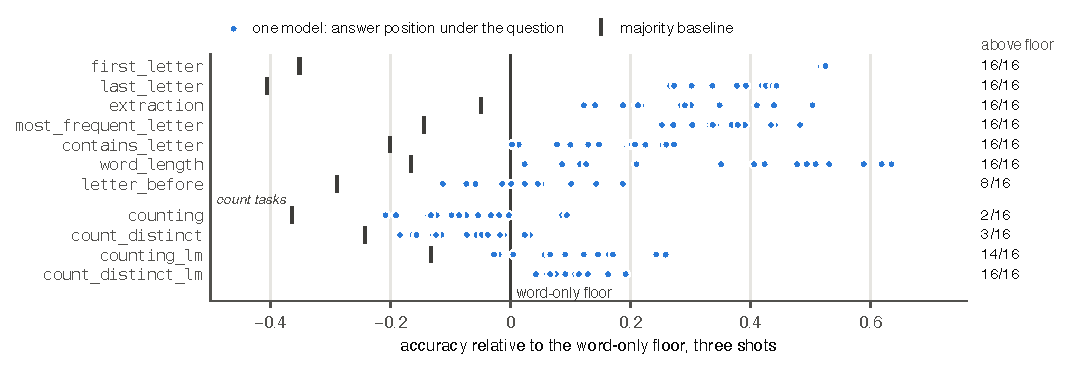
\includegraphics[width=\linewidth]{fig_nuisance.pdf}
  \caption{Word-only nuisance floors at three shots. Each dot is one model's question-arm probe
    (answer position, held-out layer selection), relative to the task's word-only floor (vertical
    line); the bar marks the majority baseline relative to the same floor (for
    \texttt{count\_distinct\_lm} the two coincide). Right: models above the floor. Below the gap:
    the original count tasks and their designed replacements. Floors, floor predictors and the best
    model per task are in Table~\ref{tab:nuisance}.}
  \label{fig:nuisance}
\end{figure}

\paragraph{The original count tasks fail.}
\texttt{counting} clears its floor in 2 of 16 models and \texttt{count\_distinct} in 3. The cause is
our own sampling. Stratifying \texttt{counting} by the true count made long words predict high
counts, because a letter occurring three times needs a long word; length alone predicts the answer at
0.439 against a 0.311 majority. \texttt{count\_distinct} has the same problem, since the number of
distinct letters is bounded by word length (length alone: 0.532).

\paragraph{Length matching is not enough.}
We first rebuilt the count tasks with equal numbers of examples in every (word length, answer) cell,
which makes length statistically independent of the answer. For \texttt{counting} this left the floor
at 0.61, because two other shortcuts remained. The query letter alone predicted the count at 0.46
(about half of the three-occurrence items query \texttt{e}), and the number of repeated letters
(length minus distinct letters) predicted it at 0.59, since a word with no repeated letter can only
give a count of one.

\paragraph{Designed-out shortcuts make the task measurable.}
\texttt{counting\_lm} therefore also restricts words to exactly two repeated letters and draws the
query letter uniformly within each cell from letters that occur at every count at that length
(Appendix~\ref{app:lm}). Length, repetition and query-letter predictors then sit near the majority
baseline (0.25, 0.27 and 0.22 against 0.27), and the floor falls to 0.404, set by the letter set.
\texttt{counting\_lm} clears it in 14 of 16 models at three shots (16 of 16 at zero shots), by up to
$+0.259$. \texttt{count\_distinct\_lm} draws equal numbers per cell over lengths 8--9 and answers 5--8;
its only informative word predictor, the letter set, determines the answer and is excluded, so its
floor equals the majority baseline and it tests above-majority decodability only.

\paragraph{The rebuilt count tasks are only partly question-driven.}
Without the question, \texttt{counting\_lm} keeps about half of its above-floor signal (0.48--0.52,
neutral carrier) and \texttt{count\_distinct\_lm} two thirds or more (0.67--0.91,
Table~\ref{tab:retained}). Neither shows a significant question$\times$scale interaction
(\texttt{counting\_lm}: $p = 0.25$ and $0.12$ at zero and three shots; \texttt{count\_distinct\_lm}:
$p = 0.97$ and $0.06$). Removing a confound turned the count tasks from unmeasurable into measurable,
but not into further instances of the late, scale-dependent signal of \S\ref{sec:question}.

\paragraph{Other tasks.}
Six tasks clear their floors in every model by large margins. \texttt{letter\_before} clears it in 8 of
16 models at three shots and 3 of 16 at zero shots, and we treat it as marginal throughout.
\texttt{extraction}'s floor is low (0.171) because position-free letter information says little about
which position was asked.
